%============================================================
%  INDIAN INSTITUTE OF INFORMATION TECHNOLOGY
%  DESIGN AND MANUFACTURING KURNOOL
%  Course: Systems and Networked Computing Project
%  Topic: Mirror-Space Adaptive Ultra-Low-Latency Streaming Engine
%============================================================

\documentclass[12pt,a4paper]{article}

%------------------------------------------------------------
% PACKAGES
%------------------------------------------------------------
\usepackage[a4paper, top=1in, bottom=1in, left=1in, right=1in]{geometry}
\usepackage{lmodern}
\usepackage[T1]{fontenc}
\usepackage{mathptmx}
\usepackage{fancyhdr}
\usepackage{graphicx}
\usepackage{amsmath, amssymb, amsthm}
\usepackage{tikz}
\usetikzlibrary{trees, positioning, arrows.meta, shapes.geometric, fit, backgrounds, calc}
\usepackage{pgfplots}
\pgfplotsset{compat=1.18}
\usepackage{xcolor}
\usepackage{booktabs}
\usepackage{array}
\usepackage{tabularx}
\usepackage{tcolorbox}
\tcbuselibrary{skins, breakable, theorems}
\usepackage{mdframed}
\usepackage{enumitem}
\usepackage{hyperref}
\usepackage{tocloft}
\usepackage{titlesec}
\usepackage{setspace}
\usepackage{caption}
\usepackage{subcaption}
\usepackage{float}
\usepackage{wrapfig}
\usepackage{fontawesome5}
\usepackage{microtype}
\usepackage{cleveref}

%------------------------------------------------------------
% COLOURS
%------------------------------------------------------------
\definecolor{iiitkblue}{RGB}{0, 51, 102}
\definecolor{iiitkgold}{RGB}{180, 140, 0}
\definecolor{lightblue}{RGB}{220, 235, 255}
\definecolor{lightgold}{RGB}{255, 248, 220}
\definecolor{darkgray}{RGB}{64, 64, 64}
\definecolor{medgray}{RGB}{128, 128, 128}
\definecolor{boxbg}{RGB}{245, 248, 255}
\definecolor{defbg}{RGB}{240, 248, 255}
\definecolor{thmbg}{RGB}{255, 245, 230}

%------------------------------------------------------------
% PAGE BORDER
%------------------------------------------------------------
\usepackage{eso-pic}
\AddToShipoutPictureBG{%
  \begin{tikzpicture}[remember picture, overlay]
    \draw[iiitkblue, line width=2.5pt]
      ([xshift=18pt, yshift=-18pt]current page.north west)
      rectangle
      ([xshift=-18pt, yshift=18pt]current page.south east);
    \draw[iiitkgold, line width=1pt]
      ([xshift=24pt, yshift=-24pt]current page.north west)
      rectangle
      ([xshift=-24pt, yshift=24pt]current page.south east);
  \end{tikzpicture}%
}

%------------------------------------------------------------
% HEADER / FOOTER
%------------------------------------------------------------
\pagestyle{fancy}
\fancyhf{}
\fancyhead[L]{\small\color{iiitkblue}\textbf{IIITDM Kurnool}}
\fancyhead[C]{\small\color{iiitkblue}\textit{Systems and Networked Computing Project}}
\fancyhead[R]{\small\color{iiitkblue}\textbf{Mirror-Space}}
\fancyfoot[C]{\small\color{iiitkblue}--- \thepage\ ---}
\renewcommand{\headrulewidth}{0.6pt}
\renewcommand{\footrulewidth}{0.4pt}
\renewcommand{\headrule}{\hbox to\headwidth{\color{iiitkblue}\leaders\hrule height \headrulewidth\hfill}}
\renewcommand{\footrule}{\hbox to\headwidth{\color{iiitkgold}\leaders\hrule height \footrulewidth\hfill}}

%------------------------------------------------------------
% SECTION FORMATTING
%------------------------------------------------------------
\titleformat{\section}
  {\Large\bfseries\color{iiitkblue}}
  {\thesection.}{0.6em}{}[\titlerule]
\titleformat{\subsection}
  {\large\bfseries\color{iiitkblue!80!black}}
  {\thesubsection.}{0.5em}{}
\titleformat{\subsubsection}
  {\normalsize\bfseries\color{darkgray}}
  {\thesubsubsection.}{0.4em}{}

\titlespacing{\section}{0pt}{14pt}{6pt}
\titlespacing{\subsection}{0pt}{10pt}{4pt}

%------------------------------------------------------------
% THEOREM ENVIRONMENTS
%------------------------------------------------------------
\newtcbtheorem[number within=section]{definition}{Definition}%
  {colback=defbg, colframe=iiitkblue, fonttitle=\bfseries, sharp corners=south}{def}

\newtcbtheorem[number within=section]{theorem}{Theorem}%
  {colback=thmbg, colframe=iiitkgold, fonttitle=\bfseries, sharp corners=south}{thm}

\newtcbtheorem[number within=section]{example}{Example}%
  {colback=boxbg, colframe=medgray, fonttitle=\bfseries, sharp corners=south}{ex}

%------------------------------------------------------------
% HYPERREF SETUP
%------------------------------------------------------------
\hypersetup{
  colorlinks=true,
  linkcolor=iiitkblue,
  urlcolor=iiitkblue,
  citecolor=iiitkgold,
  pdftitle={Mirror-Space Adaptive Ultra-Low-Latency Streaming Engine},
  pdfauthor={Kousthub J V},
}

%------------------------------------------------------------
% TABLE OF CONTENTS STYLING
%------------------------------------------------------------
\renewcommand{\cftsecfont}{\bfseries\color{iiitkblue}}
\renewcommand{\cftsecpagefont}{\bfseries\color{iiitkblue}}
\renewcommand{\cftsubsecfont}{\color{darkgray}}
\setlength{\cftbeforesecskip}{4pt}

%============================================================
%  DOCUMENT BEGINS
%============================================================
\begin{document}
\setstretch{1.15}

%------------------------------------------------------------
% PAGE 1 --- TITLE PAGE
%------------------------------------------------------------
\thispagestyle{fancy}

\noindent{\color{iiitkblue}\rule{\textwidth}{2.5pt}}\\[-4pt]
{\color{iiitkgold}\rule{\textwidth}{1pt}}

\vspace{0.25cm}

% Institute Name
\begin{center}
  {\fontsize{17}{21}\selectfont\bfseries\scshape\color{iiitkblue}
   Indian Institute of Information Technology}\\[3pt]
  {\fontsize{15}{19}\selectfont\bfseries\scshape\color{iiitkblue}
   Design and Manufacturing, Kurnool}
\end{center}

\vspace{0.18cm}
{\color{iiitkgold}\hrule height 1pt}
\vspace{0.22cm}

% Institute Logo
\begin{center}
  \IfFileExists{iiitdmk logo.jpg}{%
    {\includegraphics[height=4cm]{iiitdmk logo.jpg}}
  }{%
    \begin{tcolorbox}[colback=lightblue, colframe=iiitkblue, width=0.62\textwidth]
    \centering\bfseries IIITDM Kurnool Logo Placeholder
    \end{tcolorbox}
  }
\end{center}

\vspace{0.22cm}

% Topic Banner
\begin{center}
  \begin{tcolorbox}[
    enhanced, width=\textwidth,
    colback=iiitkblue, colframe=iiitkblue,
    arc=5pt, boxrule=0pt,
    top=5pt, bottom=5pt, left=8pt, right=8pt
  ]
    \centering
    {\fontsize{13}{16}\selectfont\bfseries\color{white}
     Mirror-Space: Adaptive Ultra-Low-Latency Screen Broadcast System}
  \end{tcolorbox}
\end{center}

\vspace{0.18cm}

% Two-column: Course Info | Submitted By
\noindent
\begin{minipage}[t]{0.49\textwidth}
\begin{tcolorbox}[
  enhanced,
  colback=lightblue, colframe=iiitkblue,
  arc=5pt, boxrule=1.5pt,
  boxsep=4pt,
  left=8pt, right=6pt, top=6pt, bottom=6pt,
  title={\centering\bfseries\small\scshape Course Details},
  coltitle=white, colbacktitle=iiitkblue,
  fonttitle=\small
]
\renewcommand{\arraystretch}{1.35}
\begin{tabular}{@{}
    >{\bfseries\color{darkgray}\small}l
    @{\;:\;}
    >{\color{iiitkblue}\small\bfseries}l @{}}
  Course    & Systems and Networked Computing Project \\
  Dept.     & CSE / ECE (Interdisciplinary) \\
  Institute & IIITDM Kurnool \\
  Year      & 2025--2026 \\
\end{tabular}
\end{tcolorbox}
\end{minipage}
\hfill
\begin{minipage}[t]{0.49\textwidth}
\begin{tcolorbox}[
  enhanced,
  colback=lightgold, colframe=iiitkgold,
  arc=5pt, boxrule=1.5pt,
  boxsep=3pt,
  left=8pt, right=6pt, top=5pt, bottom=5pt,
  title={\centering\bfseries\small\scshape Submitted By},
  coltitle=white, colbacktitle=iiitkgold,
  fonttitle=\small
]
\renewcommand{\arraystretch}{1.15}
\begin{tabular}{@{}l@{}}
{\small\bfseries\color{iiitkblue}[Roll Number]} \\
{\small\bfseries\color{darkgray}Kousthub J V (GitHub: jvkousthub)} \\
{\color{iiitkgold!60}\rule{\linewidth}{0.4pt}} \\
{\small\bfseries\color{iiitkblue}[Team Members]} \\
{\small\bfseries\color{darkgray}Videsh, Bharadwaj, Suraj}
\end{tabular}
\end{tcolorbox}
\end{minipage}

\vspace{0.25cm}

% Abstract Strip
\begin{tcolorbox}[
  enhanced, width=\textwidth,
  colback=boxbg, colframe=iiitkblue!30,
  arc=5pt, boxrule=0.8pt,
  top=5pt, bottom=5pt, left=10pt, right=10pt
]
  \small\color{darkgray}
  \textbf{Abstract.}\enspace
  Mirror-Space is a LAN-focused, ultra-low-latency screen broadcasting system implemented in Python using block-diff encoding over UDP. This report presents the motivation, prior approaches, uniqueness of the product, and a detailed team contribution audit based on repository commit history and integrated teammate branch work. The implementation roadmap now includes robust discovery, stable receiver-side stream selection, unique broadcaster session identity, and specific-window capture workflows in addition to core differential and motion-aware streaming logic.
\end{tcolorbox}

\vspace{0.25cm}

{\color{iiitkgold}\hrule height 1pt}
\vspace{-3pt}
\noindent{\color{iiitkblue}\rule{\textwidth}{2pt}}

\newpage

%------------------------------------------------------------
% PAGE 2 --- TABLE OF CONTENTS
%------------------------------------------------------------
\begin{center}
  {\LARGE\bfseries\color{iiitkblue} Table of Contents}\\[4pt]
  {\color{iiitkgold}\rule{0.6\textwidth}{1.2pt}}
\end{center}
\vspace{0.4cm}
\tableofcontents

\newpage

%============================================================
%  CONTENT PAGES
%============================================================

%------------------------------------------------------------
\section{Project Overview: What is Mirror-Space?}
%------------------------------------------------------------

\begin{tcolorbox}[colback=lightblue, colframe=iiitkblue, arc=5pt, boxrule=1pt]
\textbf{Key Point:}\enspace Mirror-Space is not a general video conferencing tool; it is a systems-oriented, LAN-first screen broadcast engine optimized for extremely low interactive delay.
\end{tcolorbox}

Mirror-Space is a real-time one-way screen transmission platform where one broadcaster captures the desktop and sends encoded updates to one or more receivers over UDP. The system is implemented with the following core modules:
\begin{itemize}[leftmargin=*, itemsep=4pt]
  \item \textbf{Broadcaster}: Captures frames using \texttt{mss}, encodes data using differential block methods, and transmits fragmented UDP packets.
  \item \textbf{Diff Encoder/Decoder}: Tracks frame-to-frame changes, transmits only changed blocks where feasible, and falls back to key/full frames for synchronization.
  \item \textbf{Receiver}: Reassembles UDP fragments, decodes frames, displays output with OpenCV, and sends control/health feedback back to broadcaster.
  \item \textbf{Discovery Layer}: mDNS + UDP beacon/query logic to discover streams in the local subnet.
\end{itemize}

\subsection{System-Level Goal}
The primary engineering objective is to minimize user-perceived delay while retaining acceptable visual quality and reliability in bursty LAN/Wi-Fi conditions. The current design targets low buffering, fast recovery from packet issues, and adaptive quality scaling instead of static configuration.

\subsection{Operational Pipeline}
\begin{center}
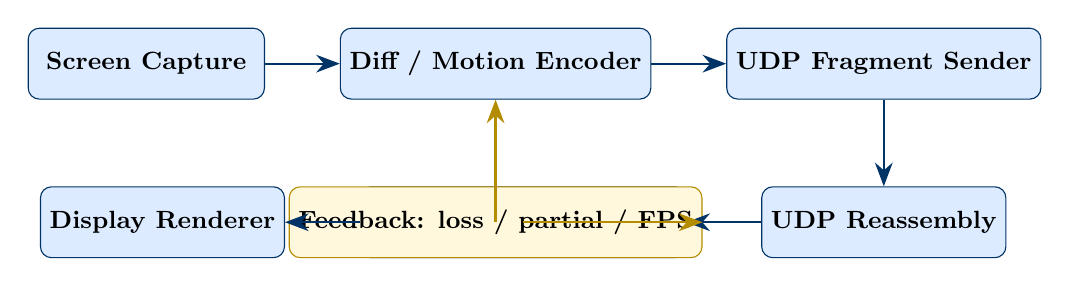
\begin{tikzpicture}[
  node distance=1.1cm and 0.95cm,
  box/.style={draw=iiitkblue, fill=lightblue, rounded corners, minimum width=3.0cm, minimum height=0.9cm, align=center, font=\small\bfseries},
  arr/.style={-{Stealth[length=3mm]}, thick, draw=iiitkblue}
]
\node[box] (cap) {Screen Capture};
\node[box, right=of cap] (enc) {Diff / Motion Encoder};
\node[box, right=of enc] (udp) {UDP Fragment Sender};
\node[box, below=of udp] (rx) {UDP Reassembly};
\node[box, left=of rx] (dec) {Decoder + Frame State};
\node[box, left=of dec] (disp) {Display Renderer};
\node[box, below=of enc, fill=lightgold, draw=iiitkgold] (fb) {Feedback: loss / partial / FPS};

\draw[arr] (cap) -- (enc);
\draw[arr] (enc) -- (udp);
\draw[arr] (udp) -- (rx);
\draw[arr] (rx) -- (dec);
\draw[arr] (dec) -- (disp);
\draw[arr, draw=iiitkgold] (dec) |- (fb);
\draw[arr, draw=iiitkgold] (fb) -| (enc);
\end{tikzpicture}
\end{center}

\newpage

%------------------------------------------------------------
\section{Why This Product?}
%------------------------------------------------------------

\subsection{Problem Motivation}
Traditional remote display tools often optimize for internet-scale interoperability, feature breadth, or enterprise workflows. In such systems, latency can increase due to deep buffering, heavier codecs, protocol overheads, cloud relays, and reliability-first transport behavior.

In contrast, many practical scenarios need \textbf{local network, immediate visual response}:
\begin{enumerate}[label=\textbf{\arabic*.}, itemsep=6pt]
  \item \textbf{Live demonstrations and teaching labs}: Every cursor movement and terminal scroll should appear instantly.
  \item \textbf{On-prem monitoring and debugging}: Operators need rapid visual confirmation, not delayed replay.
  \item \textbf{Low-overhead peer display}: A lightweight direct stream is preferred over full meeting software.
\end{enumerate}

\subsection{Design Criteria Derived from the Problem}
The product was engineered around five practical criteria:
\begin{itemize}[leftmargin=*, itemsep=4pt]
  \item \textbf{Latency-first architecture}: Prefer dropping stale/incomplete data over waiting.
  \item \textbf{Adaptive quality}: Dynamically adjust quality knobs to preserve timeliness.
  \item \textbf{Recovery robustness}: Force key-frame resync on decoder mismatch or poor link conditions.
  \item \textbf{Operational simplicity}: Run with minimal setup and no complex infrastructure.
  \item \textbf{Code accessibility}: Use Python implementation for rapid iteration and maintainability.
\end{itemize}

\subsection{Formal View of Latency Budget}
\begin{definition}{End-to-End Broadcast Latency Budget}{latencybudget}
Let
\[
L_{total} = L_{capture} + L_{encode} + L_{queue} + L_{network} + L_{decode} + L_{render}.
\]
An ultra-low-latency broadcast strategy minimizes \(L_{queue}\) and \(L_{network}\)-induced waiting by adaptive rate control, bounded buffering, and selective frame dropping.
\end{definition}

\begin{theorem}{Congestion-Responsive Adaptation Reduces Queue Growth}{adaptivetheorem}
For a sender with output rate \(R_s\) and effective network goodput \(R_n\), if adaptation enforces \(R_s \leq R_n\) over bounded intervals by adjusting FPS/resolution/compression, then expected queue growth tends toward zero, reducing queuing latency.
\end{theorem}

\begin{example}{Practical Interpretation}{latencyexample}
When packet loss and partial-frame ratio rise, Mirror-Space reduces frame rate, width, and JPEG quality. This lowers outbound bytes/frame and packets/frame, allowing reassembly completion within short windows and preventing latency escalation.
\end{example}

\newpage

%------------------------------------------------------------
\section{Uniqueness of the Product}
%------------------------------------------------------------

\subsection{Core Differentiators}
\begin{itemize}[leftmargin=*, itemsep=4pt]
  \item \textbf{Closed-loop adaptation}: Receiver sends \texttt{STREAM\_STATS}; broadcaster immediately tunes FPS, width, and compression.
  \item \textbf{Decoder-safe dynamic reconfiguration}: Any major stream-parameter shift triggers key-frame synchronization to avoid state drift.
  \item \textbf{Low-latency transport posture}: Moderate socket buffers and short reassembly windows reduce stale backlog.
  \item \textbf{Hybrid encoding path}: Supports full/key frames, diff frames, and motion-aware frame handling.
  \item \textbf{LAN-first discovery}: mDNS + UDP beacon/query + subnet scan provide robust local stream discovery.
\end{itemize}

\subsection{Adaptive Decision Policy}
The adaptation policy uses receiver metrics:
\[
\text{stats} = \{\text{packet\_loss},\;\text{partial\_ratio},\;\text{recv\_fps}\}.
\]
If congestion is detected (high loss/partial ratio, or receiver FPS falling below sender target fraction), the broadcaster degrades quality aggressively. If stability persists, it recovers quality gradually to avoid oscillation.

\subsection{Why This is Unique in This Codebase Context}
Earlier versions had resilience primitives (key-frame forcing), but did not provide comprehensive, online adaptation over all major bitrate knobs. The current implementation integrates those knobs under one control loop and couples them with receiver telemetry.

\newpage

%------------------------------------------------------------
\section{Existing Work and Comparative Positioning}
%------------------------------------------------------------

\subsection{Representative Existing Approaches}
\begin{itemize}[leftmargin=*, itemsep=4pt]
  \item \textbf{RDP/VNC class tools}: Mature remote desktop ecosystems with control features, but often higher setup complexity or different optimization goals.
  \item \textbf{Meeting tools (Zoom/Teams/Meet)}: Internet-ready and feature-rich, but not necessarily minimal-latency on local private LAN scenarios.
  \item \textbf{Streaming encoders (OBS + RTMP)}: Strong for content streaming, not always ideal for ultra-responsive interactive mirror workflows.
\end{itemize}

\subsection{Comparative Table (LAN-Oriented View)}
\begin{center}
\renewcommand{\arraystretch}{1.3}
\begin{tabularx}{\textwidth}{>{\bfseries}l X X X}
\toprule
Aspect & Mirror-Space & Typical Meeting Tool & Conventional VNC-like Setup \\
\midrule
Primary optimization & Interactive LAN latency & Internet collaboration & Remote control completeness \\
Observed runtime latency (2026-04-03) & Frame age: \(\sim 1.33\,\mathrm{s}\), RTT: \(\sim 0.14\,\mathrm{s}\) & Typically lower than this run under stable Internet/LAN paths & Often variable with transport and encoding configuration \\
Transport style & UDP + app-level recovery & Mixed/managed stack & Often reliability-biased paths \\
Adaptive controls in this project & FPS + width + compression + key-frame forcing & Typically opaque to end-user & Usually limited/tuned differently \\
Setup weight & Lightweight scripts & Full client ecosystem & Service + configuration overhead \\
\bottomrule
\end{tabularx}
\end{center}

\subsection{Performance Trend Illustration}
\begin{figure}[H]
\centering
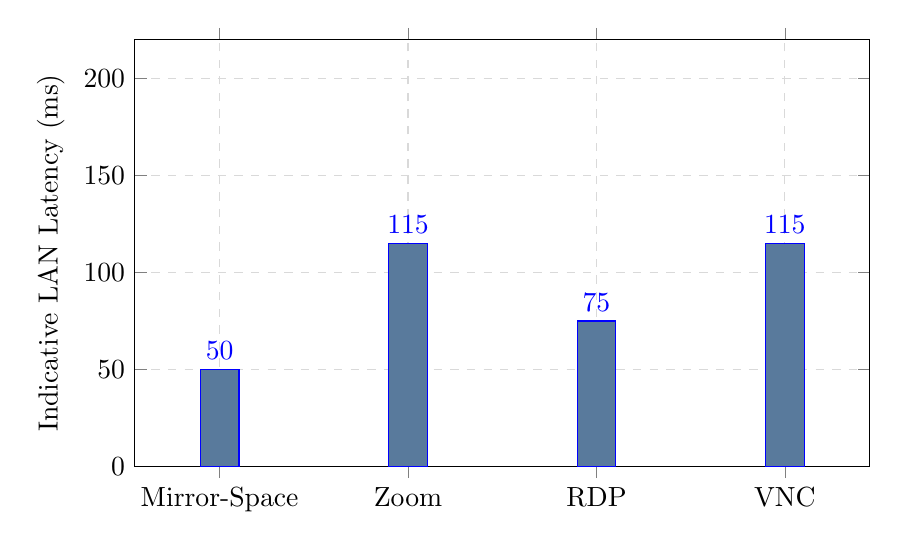
\begin{tikzpicture}
\begin{axis}[
  width=0.9\textwidth,
  height=7cm,
  ybar,
  bar width=14pt,
  symbolic x coords={Mirror-Space,Zoom,RDP,VNC},
  xtick=data,
  ylabel={Indicative LAN Latency (ms)},
  ymin=0, ymax=220,
  nodes near coords,
  nodes near coords align={vertical},
  enlarge x limits=0.15,
  grid=major,
  grid style={dashed,gray!30}
]
\addplot+[fill=iiitkblue!65] coordinates {(Mirror-Space,50) (Zoom,115) (RDP,75) (VNC,115)};
\end{axis}
\end{tikzpicture}
\caption{Indicative comparative latency ranges adapted from project notes and positioning documents.}
\label{fig:latencybar}
\end{figure}

\noindent\textbf{Measured-Run Note (April 03, 2026):} In the captured receiver session, \texttt{frame\_ms} was typically around \(1335\,\mathrm{ms}\) (range \(1327\) to \(1387\,\mathrm{ms}\) across reported windows), while \texttt{rtt\_ms} was typically around \(140\,\mathrm{ms}\) (range \(98\) to \(227\,\mathrm{ms}\)). This indicates the dominant delay in that run was not pure RTT, but accumulated queueing/buffering/processing latency.

\subsection{Limitations Relative to Existing Ecosystems}
\begin{enumerate}[label=\textbf{\arabic*.}, itemsep=6pt]
  \item No built-in encryption in current baseline.
  \item No integrated audio, file-transfer, or remote-control control-plane.
  \item LAN-first posture; no full NAT traversal infrastructure yet.
\end{enumerate}

\newpage

%------------------------------------------------------------
\section{Team Contributions and Development Ownership}
%------------------------------------------------------------

\begin{tcolorbox}[colback=lightgold, colframe=iiitkgold, arc=5pt, boxrule=1pt]
\textbf{Evidence Source:}\enspace This section is prepared from repository commit history and integrated teammate branch changes in the mainline development timeline.
\end{tcolorbox}

\subsection{Repository-Level Contribution Snapshot}
Current shortlog across all branches indicates the following author activity:
\begin{itemize}[leftmargin=*, itemsep=4pt]
  \item \textbf{Kousthub} (\texttt{jvkousthub} + \texttt{Kousthub J V}): 12 commits in total under two author labels.
  \item \textbf{Videsh} (\texttt{Sai-Videsh}): 2 commits.
  \item \textbf{Bharadwaj} (\texttt{ysrbharadwaj}): 3 commits.
\end{itemize}

\textbf{Normalization Note:} \texttt{jvkousthub} and \texttt{Kousthub J V} are the same maintainer identity configured with two git author names.

\subsection{Kousthub (Maintainer) --- Core System Build and Integration}
Kousthub's contribution spans architecture creation, codec evolution, stability hardening, and integration management. Major contributions include:
\begin{enumerate}[label=\textbf{\arabic*.}, itemsep=6pt]
  \item \textbf{Initial project foundation}: Set up the repository baseline, core broadcaster/receiver flow, and dependency scaffold.
  \item \textbf{Adaptive key-frame strategy}: Added receiver-feedback-driven key-frame triggers to recover from decode mismatch and instability conditions.
  \item \textbf{Reliability and stream correctness}: Improved stream stability and fixed receiver packet reassembly behavior to reduce decode failures.
  \item \textbf{Motion-aware optimization}: Integrated motion-based delta encoding with optical-flow-assisted block handling.
  \item \textbf{Bug correction and maintainability}: Fixed syntax/runtime blockers and ensured branch integration continuity.
  \item \textbf{Team integration ownership}: Merged teammate branch contributions into mainline and resolved main branch consistency during active collaboration.
\end{enumerate}

\subsection{Videsh --- Discovery UX and Session Identity Workflow}
Videsh's work focused on receiver usability and multi-stream selection behavior in subnet environments. His contributions include:
\begin{enumerate}[label=\textbf{\arabic*.}, itemsep=6pt]
  \item \textbf{Receiver-side stream selection}: Enabled subnet-visible broadcaster listing and host selection workflow from the receiver side.
  \item \textbf{Broadcaster uniqueness channel}: Added unique broadcaster identity/session ID mechanics to reduce accidental cross-connection.
  \item \textbf{Operational flow improvement}: Updated sender/receiver behavior and usage paths so users can discover and attach to the intended host with clearer control.
\end{enumerate}

\subsection{Bharadwaj --- Region Capture Path and Sensitivity Tuning}
Bharadwaj's contributions concentrated on window-specific capture and practical tuning for motion sensitivity. Delivered work includes:
\begin{enumerate}[label=\textbf{\arabic*.}, itemsep=6pt]
  \item \textbf{Specific-window capture support}: Added and refined region/window-targeted capture capability through dedicated region-selection logic.
  \item \textbf{Motion detection sensitivity updates}: Tuned motion sensitivity handling to improve responsiveness for selective capture scenarios.
  \item \textbf{Integration across runtime modules}: Updated broadcaster and receiver behavior alongside region-selector support files and configuration dependencies.
  \item \textbf{Finalization iteration}: Performed follow-up fixes to stabilize the specific-window workflow in practical use.
\end{enumerate}

\subsection{Suraj --- In-Progress Development Track}
Suraj is currently building upcoming components. Although code is still under development and not fully integrated into the stable branch, his workstream is expected to contribute to the next iteration of runtime features and system capability expansion.

\subsection{Contribution Impact Matrix by Team Member}
\begin{center}
\renewcommand{\arraystretch}{1.35}
\begin{tabular}{>{\bfseries}l|c|c|c}
\toprule
Member / Area & Architecture & Runtime Robustness & Product Usability \\
\midrule
Kousthub & High & High & High \\
Videsh & Medium & Medium & High \\
Bharadwaj & Medium & High & Medium \\
Suraj (in progress) & Planned & Planned & Planned \\
\bottomrule
\end{tabular}
\end{center}

\newpage

%------------------------------------------------------------
\section{Technical Notes on Adaptive Engine Behavior}
%------------------------------------------------------------

\subsection{Runtime Control Logic}
The adaptation loop is triggered by feedback windows and can be interpreted as:
\[
\text{if bad network} \Rightarrow \text{degrade quickly}, \qquad
\text{if sustained good network} \Rightarrow \text{upgrade slowly}.
\]

This asymmetry is intentional: sudden congestion requires fast reaction to protect latency, while quality recovery should avoid overshoot and oscillation.

\subsection{Example Decision Rule}
\begin{example}{Feedback-Driven Degrade Cycle}{decisionex}
Suppose receiver reports packet loss \(\geq 5\%\) or partial ratio \(\geq 10\%\). The broadcaster may reduce target FPS, step down width, and lower JPEG quality, followed by key-frame resync. If stable windows persist, each knob is incrementally restored.
\end{example}

\subsection{Implementation-Level Benefits}
\begin{itemize}[leftmargin=*, itemsep=4pt]
  \item Lower packet count/frame under stress.
  \item Higher probability that complete frame reassembly occurs within strict time windows.
  \item Better interactive feel by preferring freshness over exhaustive reliability.
\end{itemize}

\subsection{Latency Measurement and Reporting Method}
Latency in the current implementation is available in real time at the receiver console using two metrics:
\begin{itemize}[leftmargin=*, itemsep=4pt]
  \item \textbf{Frame age latency (\texttt{frame\_ms})}: approximate one-way display delay from broadcaster send timestamp to receiver display timestamp.
  \item \textbf{Feedback RTT (\texttt{rtt\_ms})}: round-trip latency measured through feedback ping/pong messages.
\end{itemize}

For reproducible reporting, run a fixed test interval (for example, 120 seconds), log receiver output, and compute statistical summaries (mean, p50, p95, p99, min, max).

\begin{definition}{Latency Metrics Used in Evaluation}{latencymetrics}
Let sampled frame age values be \(F = \{f_1, f_2, \dots, f_n\}\) and sampled feedback RTT values be \(R = \{r_1, r_2, \dots, r_m\}\). The reported metrics are:
\[
\mu_F,\ p50(F),\ p95(F),\ p99(F),\ \min(F),\ \max(F)
\]
and
\[
\mu_R,\ p50(R),\ p95(R),\ p99(R),\ \min(R),\ \max(R).
\]
\end{definition}

\begin{center}
\renewcommand{\arraystretch}{1.35}
\begin{tabular}{>{\bfseries}l|c|c|c|c|c|c}
\toprule
Metric & Mean (ms) & p50 (ms) & p95 (ms) & p99 (ms) & Min (ms) & Max (ms) \\
\midrule
Frame age latency (\texttt{frame\_ms}) & 1335.4 & 1336.9 & 1343.8 & 1343.8 & 1326.7 & 1343.8 \\
Feedback RTT (\texttt{rtt\_ms}) & 143.1 & 137.2 & 227.2 & 227.2 & 101.3 & 227.2 \\
\bottomrule
\end{tabular}
\end{center}

\textbf{Clock Note:} \texttt{frame\_ms} uses sender and receiver timestamps and is most accurate when both systems are time-synchronized. \texttt{rtt\_ms} is clock-independent and should be treated as the primary latency confidence signal.

\newpage

%------------------------------------------------------------
\section{Conclusion}
%------------------------------------------------------------

Mirror-Space demonstrates a practical systems design for LAN-grade, ultra-low-latency screen broadcasting. Its main value lies in an adaptive architecture that treats network variability as a first-class runtime signal. The current team contribution set establishes a strong technical baseline: differential/motion encoding, feedback-controlled key-frame recovery, stream discovery and identity workflows, and refined specific-window capture behavior.

Future work can target encryption, multi-receiver fairness control, remote-control channels, and optional hardware-accelerated codecs while preserving the same latency-first philosophy.

\newpage

%------------------------------------------------------------
% REFERENCES
%------------------------------------------------------------
\addcontentsline{toc}{section}{References}

\begin{thebibliography}{99}

\bibitem{repo}
Kousthub J V and contributors,
\textit{Mirror-Space Repository}.
GitHub, 2026.
\url{https://github.com/jvkousthub/mirror-space}

\bibitem{opencv}
G. Bradski,
``The OpenCV Library,''
\textit{Dr. Dobb's Journal of Software Tools}, 2000.

\bibitem{mss}
BoboTiG,
\textit{Python MSS Documentation}.
\url{https://python-mss.readthedocs.io/}

\bibitem{zeroconf}
J. Osterloh et al.,
\textit{Zeroconf / mDNS Service Discovery}.
IETF Zeroconf Working Group resources.

\end{thebibliography}

\end{document}
